\documentclass[aspectratio=169, 10pt]{beamer}
\usetheme{Madrid}
\usefonttheme{professionalfonts}

\usepackage[utf8]{inputenc}
\usepackage[english]{babel}
\usepackage[linguistics]{forest}
\usepackage{algorithmic}
\usepackage{amsfonts}
\usepackage{amsmath}
\usepackage{amssymb}
\usepackage{array}
\usepackage{bookmark}
\usepackage{caption}
\usepackage{colortbl}
\usepackage{csquotes}
\usepackage{graphicx}
\usepackage{hyperref}
\usepackage{lipsum}
\usepackage{lmodern}
\usepackage{mathptmx}
\usepackage{mathtools}
\usepackage{svg}
\usepackage{xcolor}
\usepackage{multirow}

\hypersetup{
    colorlinks=true,
    linkcolor=blue,
    filecolor=blue,      
    urlcolor=blue,
}

\title{Tutorial 2}
\subtitle{Decision Tree, Cross-validation, Precision and Recall}
\author{Luke Chang}
\institute{The University of Auckland}
\date{Mar. 2021}


\begin{document}

\frame{\titlepage}

%-------------------------------------------------------------------------------
\begin{frame}
    \frametitle{Objectives}
    
    \begin{enumerate}
        \item Evaluation Metrics: Accuracy, Precision, Recall and F1 score
        \item ROC curve and AUC
        \item Should you trust the results?
        \item Parametric Tests VS. Non-parametric Tests
        \item Regression and Least Square Problem
        \item Ensemble Methods
    \end{enumerate}
    
\end{frame}

%-------------------------------------------------------------------------------
\begin{frame}
    \frametitle{Confusion Matrix}
    
    Confusion Matrix can be applied to \textbf{binary} classification as well as for \textbf{multiclass} classification problems.
            
    \begin{table}[]
        \begin{tabular}{cccc}
                                         &                                        & \multicolumn{2}{c}{\textbf{Predicted}}                                    \\
                                         &                                        & \textbf{Positive}                   & \textbf{Negative}                   \\ \cline{3-4} 
        \multirow{2}{*}{\textbf{Actual}} & \multicolumn{1}{c|}{\textbf{Positive}} & \multicolumn{1}{c|}{\cellcolor{blue!25}True Positive}  & \multicolumn{1}{c|}{\cellcolor{red!25}False Negative} \\ \cline{3-4} 
                                         & \multicolumn{1}{c|}{\textbf{Negative}} & \multicolumn{1}{c|}{\cellcolor{red!25}False Positive} & \multicolumn{1}{c|}{\cellcolor{blue!25}True Negative}  \\ \cline{3-4} 
        \end{tabular}
    \end{table}

    \begin{itemize}
        \item True Positive (TP): Correctly classified.
        \item True Negative (TN): Correctly rejected.
        \item False Positive (FP): Incorrectly classified. Type I Error.
        \item False Negative (FN): Incorrectly rejected. Type II Error.
    \end{itemize}

    \[
        \text{Accuracy} = \frac{\text{TP} + \text{TN}}{\text{TP} + \text{TN} + \text{FP} + \text{FN}}
    \]

\end{frame}

%-------------------------------------------------------------------------------
\begin{frame}
    \frametitle{Confusion Matrix}

    How many selected items are relevant? $\text{Selected Elements} = \text{TP}+ \text{FP}$
    \[
        \text{Precision (P)} = \frac{\text{TP}}{\text{TP}+ \text{FP}}
    \]

    How many relevant items are selected? $\text{Relevant Elements} = \text{TP}+ \text{FN}$
    \[
        \text{Recall (R)} = \frac{\text{TP}}{\text{TP}+ \text{FN}}
    \]
    
    $F_1$ score is the \textbf{harmonic mean} between Precision and Recall.

    \[
        F_1 = 2 \times \frac{P \times R}{P + R}
    \]
    
\end{frame}

%-------------------------------------------------------------------------------
\begin{frame}
    \frametitle{Example -- Weather Prediction}
    \begin{columns}
        \begin{column}{0.5\textwidth}
            Build a logistic regression model to predict the weather based on the humidity. \\
            Recorded 10 days in total.
            \begin{table}[]
                \begin{tabular}{cc}
                \textbf{Class} & \textbf{Prediction} \\ \hline
                P              & P                   \\
                N              & P                   \\
                P              & N                   \\
                P              & P                   \\
                N              & P                   \\
                P              & P                   \\
                N              & P                   \\
                N              & N                   \\
                N              & N                   \\
                P              & P                  
                \end{tabular}
            \end{table}

            \textbf{Caveat:} A model with high Recall may also has high FPR (Type I Error).

        \end{column}
        \begin{column}{0.5\textwidth}
            \begin{table}[]
                \begin{tabular}{ccccc}
                \textbf{}                        & \textbf{}                       & \multicolumn{2}{c}{\textbf{Predicted}}          &                \\
                                                 &                                 & \textbf{P}             & \textbf{N}             & \textbf{Total} \\ \cline{3-4}
                \multirow{2}{*}{\textbf{Actual}} & \multicolumn{1}{c|}{\textbf{P}} & \multicolumn{1}{c|}{4} & \multicolumn{1}{c|}{1} & 5              \\ \cline{3-4}
                                                 & \multicolumn{1}{c|}{\textbf{N}} & \multicolumn{1}{c|}{3} & \multicolumn{1}{c|}{2} & 5              \\ \cline{3-4}
                                                 & \textbf{Total}                  & 7                      & 3                      & \textbf{10}   
                \end{tabular}
            \end{table}
            
            \[
                \text{Acc.} = \frac{6}{10} = 0.6
            \]

            \[
                \text{Precision (P)} = \frac{\text{TP}}{\text{TP}+ \text{FP}} = \frac{4}{4+3} \approx 0.571
            \]

            \[
                \text{Recall (R)} = \frac{\text{TP}}{\text{TP}+ \text{FN}} = \frac{4}{4+1} \approx 0.8
            \]

            \[
                F_1 = 2 \frac{P \times R}{P + R} = 2 \times \frac{0.571 \times 0.8}{0.571 + 0.8} \approx 0.667
            \]

        \end{column}
    \end{columns}

\end{frame}

%-------------------------------------------------------------------------------
\begin{frame}
    \frametitle{Precision-Recall (PR) Curve (Optional)}
    
    Average precision (AP) summarizes such a plot as the weighted mean of precisions achieved at each threshold.
    \[
        AP = \sum_{n}(R_n - R_{n-1})P_n
    \]

    \begin{itemize}
        \item Where $P_n$ and $R_n$ are the precision and recall at the n-th threshold.
        \item A pair $(P_n, P_k)$ is referred to as an \textit{operating point}.
    \end{itemize}
    
    \begin{figure}
        \centering
        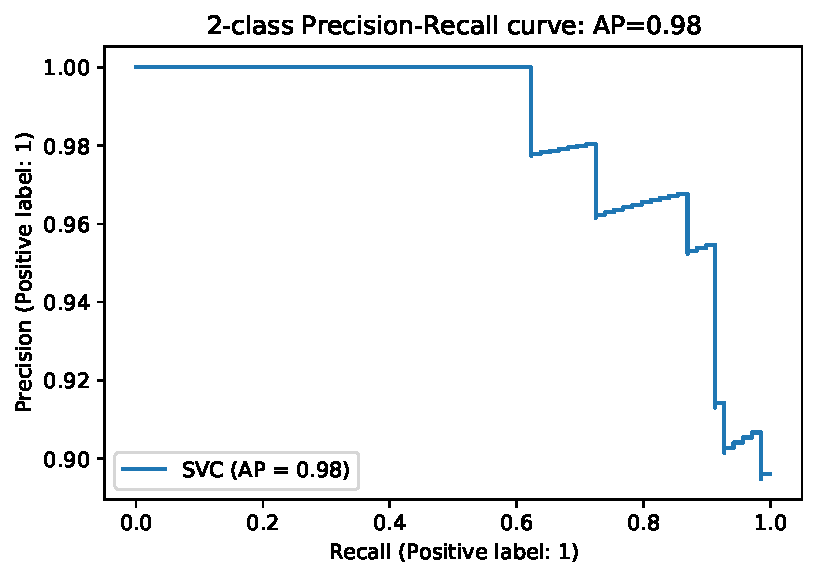
\includegraphics[width=0.35\columnwidth]{../plots/pr_curve.pdf}
        \caption{A SVM classifier trained on the Breast Cancer dataset}
    \end{figure}
\end{frame}

%-------------------------------------------------------------------------------
\begin{frame}
    \frametitle{Receiver Operating Characteristic (ROC) Curve}
    
    \begin{itemize}
        \item The ROC curve is created by plotting the true positive rate (TPR) against the false positive rate (FPR) at various threshold settings.
        \item Area Under Curve (AUC): The integration of the ROC function between 0 and 1.
    \end{itemize}
    
    \begin{figure}
        \centering
        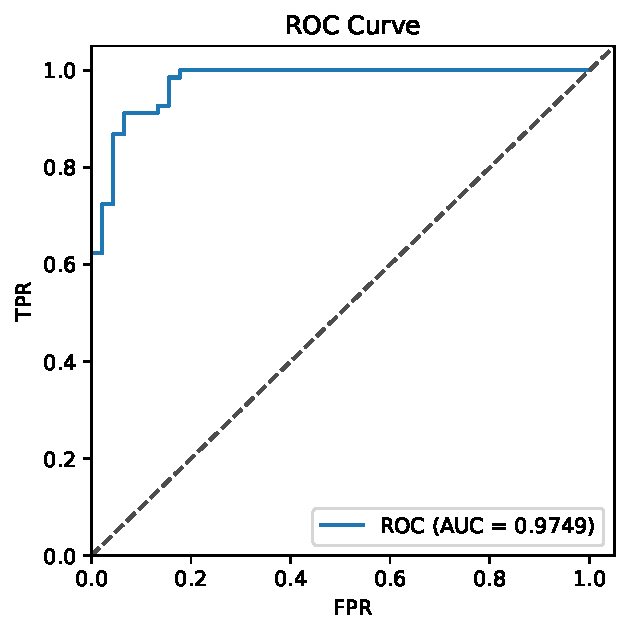
\includegraphics[width=0.3\columnwidth]{../plots/roc_curve.pdf}
        \caption{A SVM classifier trained on the Breast Cancer dataset}
    \end{figure}

\end{frame}

%-------------------------------------------------------------------------------
\begin{frame}
    \frametitle{Example -- Weather Prediction}
    \small
    
    \begin{columns}
        \begin{column}{0.5\textwidth}
            Build a logistic regression model to predict the weather based on the humidity. \\
            Recorded 10 days in total.
            
            \begin{table}[]
                \begin{tabular}{cc|cccccc}
                \textbf{}      & \textbf{}           & \multicolumn{6}{l}{\textbf{Thresholds}}                                             \\
                \textbf{Class} & \textbf{Prediction} & \textbf{0} & \textbf{0.2} & \textbf{0.4} & \textbf{0.6} & \textbf{0.8} & \textbf{1} \\ \hline
                P              & 0.95                & 1          & 1            & 1            & 1            & 1            & 0          \\
                N              & 0.85                & 1          & 1            & 1            & 1            & 1            & 0          \\
                P              & 0.78                & 1          & 1            & 1            & 1            & 0            & 0          \\
                P              & 0.66                & 1          & 1            & 1            & 1            & 0            & 0          \\
                N              & 0.6                 & 1          & 1            & 1            & 1            & 0            & 0          \\
                P              & 0.55                & 1          & 1            & 1            & 0            & 0            & 0          \\
                N              & 0.53                & 1          & 1            & 1            & 0            & 0            & 0          \\
                N              & 0.52                & 1          & 1            & 1            & 0            & 0            & 0          \\
                N              & 0.51                & 1          & 1            & 1            & 0            & 0            & 0          \\
                P              & 0.4                 & 1          & 1            & 1            & 0            & 0            & 0         
                \end{tabular}
                \end{table}

        \end{column}
        \begin{column}{0.5\textwidth}
            
            Counting TP and FP:

            \begin{table}[]
                \begin{tabular}{c|cccccc}
                \textbf{Threshold} & \textbf{0} & \textbf{0.2} & \textbf{0.4} & \textbf{0.6} & \textbf{0.8} & \textbf{1} \\ \hline
                \textbf{TPR}       & 1          & 1            & 1            & 0.60         & 0.2          & 0          \\
                \textbf{FPR}       & 1          & 1            & 1            & 0.4          & 0.2          & 0         
                \end{tabular}
            \end{table}
            
            Sort the results:

            \begin{table}[]
                \begin{tabular}{c|cccccc}
                \textbf{Threshold} & \textbf{0} & \textbf{0.2} & \textbf{0.4} & \textbf{0.6} & \textbf{0.8} & \textbf{1} \\ \hline
                \textbf{TPR}       & 0          & 0.2            & 0.6            & 1         & 1         & 1          \\
                \textbf{FPR}       & 0          & 0.2           & 0.4           & 1          & 1          & 1         
                \end{tabular}
            \end{table}

            \begin{figure}
                \centering
                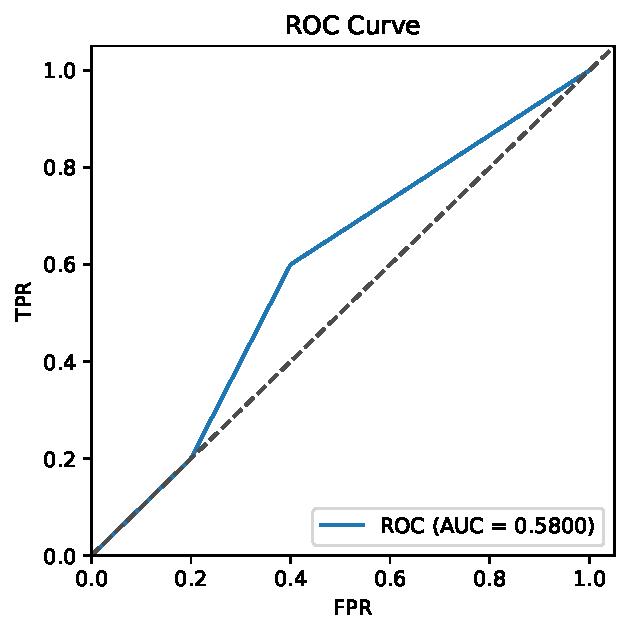
\includegraphics[width=0.4\columnwidth]{../plots/roc_curve_eg.pdf}
            \end{figure}

        \end{column}
    \end{columns}
\end{frame}

%-------------------------------------------------------------------------------
\begin{frame}
    \frametitle{Should you trust the results?}

    Scenario 1 from Page 48 in Week 2 slides

    \begin{itemize}
        \item I built a model based on the data you gave me
        \item It classified your data with 98\% accuracy
        \item It should get 98\% accuracy on the rest of your data
    \end{itemize}

    Should you trust them?\\

    \begin{itemize}
        \item They are reporting training error
        \item This might have nothing to do with test error
        \item E.g., They could have t a very deep decision tree
    \end{itemize}

    Why?

    \begin{itemize}
        \item If they only tried a few very simple models, the 98\% might be reliable
        \item E.g., They only considered decision stumps with simple 1-variable rules
    \end{itemize}
    
\end{frame}

%-------------------------------------------------------------------------------
\begin{frame}
    \frametitle{Should you trust the results?}
    
    Scenario 2 from Page 49 in Week 2 slides

    \begin{itemize}
        \item I built a model based on half of the data you gave me
        \item It classified the other half of the data with 98\% accuracy
        \item It should get 98\% accuracy on the rest of your data
    \end{itemize}

    Probably

    \begin{itemize}
        \item They computed the validation error once
        \item This is an unbiased approximation of the test error
        \item Trust them if you believe they did not violate the golden rule
    \end{itemize}

\end{frame}

%-------------------------------------------------------------------------------
\begin{frame}
    \frametitle{Should you trust the results?}
    
    Scenario 4 from Page 51 in Week 2 slides

    \begin{itemize}
        \item I built 1 billion models based on half of the data you gave me
        \item One of them classified the other half of the data with 98\% accuracy
        \item It should get 98\% accuracy on the rest of your data
    \end{itemize}

    Probably not

    \begin{itemize}
        \item They computed the validation error a huge number of times
        \item They tried so many models, one of them is likely to work by chance
    \end{itemize}

    Why?

    \begin{itemize}
        \item If the 1 billion models were all extremely-simple, 98\% might be reliable.
    \end{itemize}

\end{frame}

%-------------------------------------------------------------------------------
\begin{frame}
    \frametitle{Regression and Least Square Problem}
    
    There are $n$ samples, each sample has $d$ features
    \[
        w = \begin{bmatrix}
            w_1 \\ \vdots \\ w_d
        \end{bmatrix},
        y = \begin{bmatrix}
            y_1  \\ \vdots \\ y_n
        \end{bmatrix},
        x_i = \begin{bmatrix}
            x_1  \\ \vdots \\ x_d
        \end{bmatrix}
    \]
    
    $X$ is a matrix which represents all samples. Such that:

    \[
        \hat{y} = X w = 
        \begin{bmatrix}
            x^T_1 \\ \vdots \\ x^T_n
        \end{bmatrix} 
        \begin{bmatrix}
            w_1 \\ \vdots \\ w_d
        \end{bmatrix}
        = 
        \begin{bmatrix}
            x_{11} & \cdots & x_{1d} \\
            \vdots & \ddots & \vdots \\
            x_{n1} & \cdots & x_{nd}
        \end{bmatrix}
        \begin{bmatrix}
            w_1 \\ \vdots \\ w_d
        \end{bmatrix}
        = 
        \begin{bmatrix}
            \hat{y}_1 \\ \vdots \\ \hat{y}_n
        \end{bmatrix}
    \]

    Mean Squared Error:
    \[
        \text{MSE} = \frac{1}{n} \sum^{n}_{i=1}(y_i - \hat{y}_i)^2
    \]
\end{frame}

%-------------------------------------------------------------------------------
\begin{frame}
    \frametitle{Cross Validation Questions}
    \begin{block}{Question 1}
        If you do 2-fold cross validation, 10-fold cross validation or leave-one-out, or use a 70/30 percent train/validation single split.  What effect will this have on your results?
    \end{block}
    
    \begin{itemize}
        \item Leave-one-out means that you have a bigger training set and a bigger validation set. Also you have N repetitions where N is the size of your dataset.
        \item 2-fold gives you a much smaller training set but a bigger validation set.  A bigger validation set is good but a smaller training set is not – high bias.
        \item 10-fold validation gives you a bigger training set but an even smaller validation set than 2-fold – high variance.
    \end{itemize}

    \begin{block}{Question 2}
        Which will give you the best representative value to the “unseen test set”?
    \end{block}

    Probably leave-one-out, with 2-fold the training set might be too small and with 10-fold then validation set might be too small, but tenfold is typically better than 2-fold.

\end{frame}

%-------------------------------------------------------------------------------
\begin{frame}
    \frametitle{Cross Validation Questions}
    \begin{block}{Question 3}
        Does it matter how large your original dataset is?\\
        Will you get a different answer for a very big or a very small dataset?
    \end{block}

    \begin{itemize}
        \item For a very big dataset – all will probably give you the same answer
        \item For a very small dataset – you would probably have to do 10-fold or leave-one-out to get good results
    \end{itemize}

    \begin{block}{Question 4}
        Which will be the fastest in terms of computation?
    \end{block}

    \begin{itemize}
        \item Leave-one-out is the most expensive, you have to learn N models.
        \item 10-fold CV means you need to learn 10 models and 2-fold means you have to learn 2 models.
    \end{itemize}

\end{frame}

\begin{frame}
    \frametitle{Ensemble Questions}
    \begin{block}{Question 1}
        What are the two key factors an ensemble must have?
    \end{block}

    \begin{itemize}
        \item Each tree must perform better than random guess/ average.
        \item Must be uncorrelated.
    \end{itemize}

    \begin{block}{Question 2}
        Which will be the fastest in terms of computation?
    \end{block}

    \begin{itemize}
        \item Leave-one-out is the most expensive, you have to learn N models.
        \item 10-fold CV means you need to learn 10 models and 2-fold means you have to learn 2 models.
    \end{itemize}

\end{frame}

\begin{frame}
    \frametitle{Ensemble Questions}
    \begin{block}{Question 3}
        Does Error Correcting code work better when there are many classes or when there are few? Why? 
    \end{block}

    It will work better with many classes with 3 classes there are very few codes.

    \begin{block}{Question 4}
        4.	If you are going to choose with replacement can you then make your training set as big as you want? Will this work? 
    \end{block}

    You cannot make a million instances out of 100, but if you are short on data you can use this to try and bolster your results – especially in ensembles.

\end{frame}

\begin{frame}
    \frametitle{Ensemble Questions}
    \begin{block}{Question 5}
        What is one of the main differences between random forest and bagging?
        \onslide<2->{
            Random forest samples the features.
            }
        \begin{itemize}
            \item What will the effect be of having a dataset with a larger or smaller number of instances?\\
            \onslide<2->{
                The effect on bagging and random forest will be the same – they both sample the instance space with replacement.
            }
            \item What will the effect be of having a dataset with a larger or smaller number of features?\\
            \onslide<2->{
                Since random forests sample the features you might get better results when there are a lot of features because you got rid of a lot of noise – but with a data set with only a few features you might do worse because you are not left with enough features to make a good classifier
            }
        \end{itemize}
    \end{block}

\end{frame}

\begin{frame}
    \frametitle{Ensemble Questions}
    \begin{block}{Question 6}
        Will variable importance in Random Forest always give you the “correct” answer? Why or why not? 
    \end{block}

    \onslide<2->{
        No because if you have correlated attributes Random forest will say neither are important even if they are the most important.  This is because it randomizes the variables one at a time, thereby relying on the correlated variable when each is randomized.
    }

    \onslide<3->{
        \begin{block}{Question 7}
            Which of the “methods for constructing ensembles” does random forest use? 
        \end{block}
    }

    \onslide<4->{
        Manipulating the training set, Manipulating the input features (columns), Injecting Randomness
    }

\end{frame}

\begin{frame}
    \frametitle{Ensemble Questions}
    \begin{block}{Question 8}
        Which of the “methods for constructing ensembles” does XGBoost use?
    \end{block}

    \onslide<2->{
        Manipulating the training set, Manipulating the input features (columns), Injecting Randomness
    }

    \onslide<3->{
        \begin{block}{Question 9}
            What is one of the main differences between XG Boost and Random Forests? 
        \end{block}
    }

    \onslide<4->{
        XG Boost chooses without replacement so does not change the distribution of the dataset – also Boosting will have to use a smaller training set by definition; also RF uses democratic voting and XG Boost uses weighted voting
    }

\end{frame}

\begin{frame}
    \frametitle{Ensemble Questions}
    \begin{block}{Question 10}
        10.	What is the difference between attribute error and class error and does it have a major effect in ensembles? 
    \end{block}

    \onslide<2->{
        Attribute error is when noises is added to an input variable X and class error is when noise is added to the class Y
    }

    \onslide<3->{
        Boosting algorithm increases the weights of miss-classified data points over time, so that the next classifier will pay extra attention to get them right.
        \begin{block}{Question 11}
            What is the main difference between AdaBoost and XGBoost? 
        \end{block}
    }

    \onslide<4->{
        AdaBoost weights the data instances, and XGBoost weights the trees added into the ensemble – non-democratic voting.
    }

\end{frame}
\end{document}
